\label{method_har}

\subsection{Khai thác khả năng nhận dạng hoạt động dựa trên gia tốc kế}

Trong hơn hai thập kỷ qua, nhận dạng hoạt động của con người (Human Activity Recognition - HAR) đã trở thành hướng nghiên cứu thu hút sự quan tâm rộng rãi do ứng dụng thực tiễn ngày càng gia tăng trong các lĩnh vực như chăm sóc sức khỏe~\cite{vi2024efficient}, \cite{bui2024smart}, \cite{hong2023low}, \cite{dao2022human}, \cite{thu2022real}, theo dõi thể chất~\cite{vu2024sports}, và giám sát an toàn cá nhân~\cite{dao2025rfar}, \cite{bui2025development}. HAR không chỉ cho phép máy tính phân tích và hiểu hành vi con người từ tín hiệu cảm biến, mà còn hỗ trợ các hệ thống tương tác thông minh thích nghi với trạng thái của người dùng~\cite{vi2024efficient}.

Các hoạt động của lính cứu hỏa trong quá trình tìm kiếm và cứu nạn bên trong tòa nhà đóng vai trò then chốt trong việc đảm bảo an toàn và hiệu quả thực hiện nhiệm vụ. Trong nghiên cứu này, chúng tôi nhận dạng 8 hoạt động của nhân viên cứu hộ, bao gồm: nằm, ngồi, đứng, đi bộ, chạy bộ, lên cầu thang, xuống cầu thang và ngã. Bằng cách xác định chính xác các hoạt động này, hệ thống có thể cung cấp thông tin thời gian thực về trạng thái của từng cá nhân, hỗ trợ người chỉ huy trong việc đưa ra quyết định kịp thời và hiệu quả. Ngoài ra, dữ liệu thu thập từ việc giám sát hoạt động còn có thể được sử dụng để tối ưu hóa quy trình làm việc, phân bổ nguồn lực hợp lý và đào tạo nâng cao kỹ năng cho lực lượng cứu hộ. Khía cạnh mới của nghiên cứu này là khai thác khả năng nhận dạng hoạt động của con người từ dữ liệu cảm biến quán tính được sử dụng trong thuật toán định vị nhân viên cứu hộ. Việc sử dụng thông tin về các hành động đã thực hiện giúp tinh chỉnh và hỗ trợ thuật toán định vị.

Ba hướng tiếp cận chính cho HAR và phát hiện ngã hiện nay bao gồm: (i) phương pháp dựa trên thị giác máy tính; (ii) phương pháp sử dụng cảm biến môi trường; và (iii) phương pháp sử dụng cảm biến đeo. Phương pháp dựa trên thị giác cho phép giám sát tư thế và chuyển động thông qua hình ảnh từ camera, tuy nhiên gặp hạn chế do điều kiện ánh sáng, góc nhìn, cũng như các vấn đề về quyền riêng tư~\cite{vi2024efficient}. Đặc biệt, trong môi trường hỏa hoạn—nơi ánh sáng bị nhiễu loạn bởi khói, ngọn lửa và hơi nước—việc sử dụng camera trở nên kém hiệu quả hoặc hoàn toàn không khả thi. Ngược lại, cảm biến đeo như gia tốc kế, con quay hồi chuyển, từ trường (để định hướng), áp kế (để thay đổi độ cao) và đơn vị đo lường quán tính tích hợp trên đồng hồ thông minh hay điện thoại thông minh được đánh giá cao nhờ tính linh hoạt, giá thành thấp và không xâm phạm quyền riêng tư cá nhân~\cite{zhang2024effective}. Trong khi các hệ thống HAR dựa trên cảm biến đeo được cung cấp những lợi thế đáng kể, các phương pháp tiếp cận thay thế như hệ thống dựa trên Wi-Fi cũng đang được khám phá~\cite{lowe2022towards}. Các hệ thống này sử dụng thông tin trạng thái kênh Wi-Fi để nhận dạng hoạt động, cung cấp giải pháp không xâm phạm và bảo vệ quyền riêng tư. Tuy nhiên, chúng thường yêu cầu thiết lập phần cứng phức tạp hơn và có thể không đạt được cùng mức độ chính xác như các hệ thống dựa trên cảm biến đeo được~\cite{lowe2022towards}, \cite{ek2025comparing}.

Trong các hệ thống dựa trên cảm biến đeo, việc lựa chọn thuật toán nhận dạng và cấu trúc hệ thống đóng vai trò then chốt. Các phương pháp hiện tại thường được chia thành ba nhóm chính: (i) dựa trên ngưỡng~\cite{van2019development}, (ii) dựa trên học máy truyền thống~\cite{vi2024efficient}, \cite{bui2024smart}, \cite{hong2023low}, \cite{dao2022human}, \cite{thu2022real}, \cite{al2021towards}, \cite{chen2019detection},  và (iii) dựa trên học sâu~\cite{zhang2024effective}, \cite{yi2024fall}, \cite{soni2024cabmnet}. Các mô hình dựa trên ngưỡng và học máy thường yêu cầu trích xuất đặc trưng thủ công từ dữ liệu đầu vào, điển hình như độ lớn, năng lượng, độ lệch chuẩn hoặc các đặc trưng miền tần số. Các mô hình học máy như K-Nearest Neighbors~\cite{chen2019detection}, Decision Tree~\cite{bui2024smart}, \cite{thu2022real} và Random Forest~\cite{vi2024efficient}, \cite{al2021towards}, \cite{hong2023low}, \cite{dao2022human} thực hiện phân loại hành động hoặc phát hiện ngã dựa trên các đặc trưng đã trích xuất. Trong khi đó, các mô hình học sâu như mạng thần kinh tích chập (Convolutional Neural Networks - CNN)~\cite{zhang2024effective}, \cite{soni2024cabmnet} hoặc bộ nhớ dài-ngắn hạn (Long Short-Term Memory - LSTM)~\cite{yi2024fall}, \cite{soni2024cabmnet} có khả năng tự động học các đặc trưng ở mức cao và khai thác thông tin chuỗi thời gian trong dữ liệu, tuy nhiên thường đòi hỏi tài nguyên phần cứng lớn và khó triển khai trên thiết bị nhúng công suất thấp.

Việc phát triển các hệ thống nhận dạng hoạt động thời gian thực tích hợp trên vi điều khiển hiệu suất thấp (Low Performance Microcontroller - LPMC) đang trở thành một yêu cầu thiết yếu trong các ứng dụng tác nghiệp khẩn cấp, nơi mà thiết bị cần đảm bảo tính gọn nhẹ, tiêu thụ năng lượng thấp và khả năng xử lý tại chỗ, điển hình như trong hoạt động cứu nạn cứu hộ của lực lượng lính cứu hỏa. Tuy nhiên, bài toán đặt ra là cần đảm bảo độ chính xác của mô hình trong khi vẫn giới hạn được độ phức tạp tính toán và dung lượng bộ nhớ. Điều này đòi hỏi việc xây dựng các mô hình học máy không chỉ đạt hiệu suất phân loại cao mà còn có khả năng triển khai trên các vi điều khiển với bộ nhớ hạn chế (thường chỉ 128 đến 256~kB RAM và khoảng 1~MB Flash). Một thách thức đáng lưu ý là trong một số trường hợp, bộ xử lý hiệu suất thấp không đủ khả năng thực hiện nhận dạng trực tiếp, buộc phải truyền dữ liệu thô đến máy chủ để xử lý—điều này có thể dẫn đến lỗi truyền thông hoặc độ trễ không mong muốn. Mặt khác, sử dụng vi điều khiển hiệu suất cao hơn sẽ làm tăng đáng kể chi phí hệ thống, từ đó hạn chế khả năng triển khai thực tế ở quy mô lớn.

Thêm vào đó, mặc dù các mô hình học sâu hiện đang là xu hướng chủ đạo và thường đạt độ chính xác cao trong các bài toán phân loại, nhưng chúng thường không phù hợp để triển khai trên các nền tảng như ESP32/8266 hoặc STM32 do dung lượng mô hình vượt quá giới hạn phần cứng. Trong bối cảnh đó, các mô hình học máy cổ điển như Random Forest, XGBoost hoặc LightGBM với số lượng cây hạn chế và chiều sâu nhỏ được xem là lựa chọn hợp lý hơn vì tốc độ suy luận nhanh, tiêu thụ năng lượng thấp và dễ dàng chuyển đổi sang mã C/C++ thông qua các thư viện như \texttt{m2cgen} hoặc \texttt{micromlgen}.

Từ những nghiên cứu trước, có thể nhận thấy rằng: (i) hệ thống HAR trên thiết bị đeo là một hướng tiếp cận khả thi và hiệu quả cho các ứng dụng theo dõi trạng thái tác nghiệp của nhân viên cứu hộ trong môi trường khẩn cấp; (ii) giải pháp tối ưu cần kết hợp giữa mô hình có độ chính xác cao, kích thước nhỏ gọn và hiệu suất phù hợp để triển khai trên nền tảng vi điều khiển. Nghiên cứu này kế thừa các định hướng trên, tập trung đề xuất một quy trình xử lý học máy hiệu quả, sử dụng đặc trưng miền thời gian từ gia tốc kế, được đánh giá nghiêm ngặt qua nested–vanilla cross-validation, và cuối cùng lựa chọn mô hình XGBoost để triển khai trên thiết bị vi điều khiển hiệu suất thấp nhằm hướng đến giải pháp nhận dạng hành động theo thời gian thực trong các điều kiện tác nghiệp khắc nghiệt.

\subsubsection{Phân đoạn dữ liệu}

\begin{table}[b!]
    \centering
    \caption{Tổng hợp đặc điểm dữ liệu và mô hình trong các nghiên cứu liên quan về HAR}
    \label{related_segmentation_har}
    \begin{tabular}{p{0.137\linewidth}p{0.17\linewidth}p{0.073\linewidth}p{0.237\linewidth}p{0.091\linewidth}p{0.133\linewidth}}\hline\hline
        \multicolumn{1}{c}{\multirow{2}{*}{\textbf{Ấn phẩm}}} & \multicolumn{1}{c}{\multirow{2}{*}{\textbf{Hành động}}} & \textbf{Tần số lấy mẫu} & \multicolumn{1}{c}{\multirow{2}{*}{\textbf{Phân đoạn}}} & \textbf{Số lượng đặc trưng} & \multicolumn{1}{c}{\multirow{2}{*}{\textbf{Bộ phân loại}}}\\\hline
        
        \multirow{4}{*}{Nghiên cứu này} & 8 (nằm, ngồi, đứng, đi bộ, chạy bộ, lên cầu thang, xuống cầu thang, ngã) & \multicolumn{1}{c}{\multirow{4}{*}{100~Hz}} & \multirow{4}{*}{3 giây, chồng lấp 50~\%} & \multicolumn{1}{c}{\multirow{4}{*}{8}} & \multirow{4}{*}{XGBoost}\\\hline
        
        \multirow{3}{*}{\parbox[t]{\linewidth}{\justifying \noindent Vi \textit{et al.} - 2024~\cite{vi2024efficient}}} & 5 (ngồi, đứng, đi bộ, chạy bộ, đi cầu thang) & \multicolumn{1}{c}{\multirow{3}{*}{50~Hz}} & \multirow{3}{*}{8 giây, chồng lấp 40~\%} & \multicolumn{1}{c}{\multirow{3}{*}{4}} & \multirow{3}{*}{Random Forest}\\\hline
        
        Bui \textit{et al.} - 2024~\cite{bui2024smart} & 4 (nằm, ngồi, đứng, đi bộ) & \multicolumn{1}{c}{\multirow{2}{*}{100~Hz}} & \multirow{2}{*}{10 giây, chồng lấp 50~\%} & \multicolumn{1}{c}{\multirow{2}{*}{4}} & \multirow{2}{*}{Decision Tree}\\\hline
        
        Hong \textit{et al.} - 2023~\cite{hong2023low} & 4 (ngồi, đứng, đi bộ, chạy bộ) & \multicolumn{1}{c}{\multirow{2}{*}{50~Hz}} & \multirow{2}{*}{10 giây, chồng lấp 40~\%} & \multicolumn{1}{c}{\multirow{2}{*}{5}} & \multirow{2}{*}{Random Forest}\\\hline
        
        \multirow{3}{*}{\parbox[t]{\linewidth}{\justifying \noindent Dao \textit{et al.} - 2022~\cite{dao2022human}}} & 13 ADLs bao gồm các hành động chuyển tiếp & \multicolumn{1}{c}{\multirow{3}{*}{20~Hz}} & \multirow{3}{*}{Cửa sổ động từ 1 đến 3 giây} & \multicolumn{1}{c}{\multirow{3}{*}{12}} & \multirow{3}{*}{Random Forest}\\\hline
        
        Thu \textit{et al.} - 2022~\cite{thu2022real} & 5 (nằm, ngồi, đứng, đi bộ, chạy bộ) & \multicolumn{1}{c}{\multirow{2}{*}{1~Hz}} & \multirow{2}{*}{6 giây, chồng lấp 0~\%} & \multicolumn{1}{c}{\multirow{2}{*}{2}} & \multirow{2}{*}{Decision Tree}\\\hline\hline
    \end{tabular}
\end{table}

Để nâng cao hiệu quả nhận dạng hành động, dữ liệu cảm biến thu thập được cần được chia thành các phân đoạn tín hiệu (cửa sổ) có độ dài cố định, mỗi cửa sổ được gán một nhãn hành động duy nhất và đóng vai trò là đầu vào cho mô hình học máy. Trong nghiên cứu này, nhóm lựa chọn sử dụng cửa sổ thời gian có độ dài 3 giây và áp dụng tỉ lệ chồng lấp 50~\% đối với các hành động thường ngày (Activities of Daily Living - ADLs). Thiết kế này nhằm đảm bảo độ bao phủ chuỗi thời gian đầy đủ, đồng thời tận dụng hiệu quả thông tin hành vi đặc trưng—phù hợp với tính chất liên tục, cường độ cao và dễ biến động của các hoạt động cứu hộ, chữa cháy trong môi trường thực tế.

Đối với hành động té ngã—vốn có diễn biến ngắn, mạnh và dễ phân biệt—mỗi cửa sổ được cắt bao gồm 1,5 giây trước và 1,5 giây sau thời điểm va chạm, nhằm ghi nhận đầy đủ giai đoạn trước, trong và sau ngã. Việc chuẩn hóa độ dài cửa sổ giúp giảm thiểu nguy cơ một phân đoạn chứa nhiều hành động khác nhau, từ đó nâng cao độ chính xác và tính nhất quán của mô hình phân loại.

So với các nghiên cứu trước (Bảng~\ref{related_segmentation_har}), hầu hết các hệ thống HAR lựa chọn tần số lấy mẫu từ 20 đến 100~Hz và độ dài cửa sổ từ 2 đến 10 giây. Một số nghiên cứu sử dụng tần số thấp hơn (ví dụ: 50~Hz trong~\cite{vi2024efficient}, \cite{hong2023low}) nhằm giảm kích thước dữ liệu và tiết kiệm năng lượng, phù hợp với các ứng dụng tiêu dùng trên thiết bị nhúng có tài nguyên hạn chế. Tuy nhiên, để duy trì đủ thông tin cho huấn luyện mô hình, các nghiên cứu này phải tăng độ dài cửa sổ lên 8–10 giây. Cách tiếp cận đó có thể làm tăng xác suất một cửa sổ chứa nhiều hành động nối tiếp nhau, gây khó khăn cho phân loại theo thời gian thực. Điều này đặc biệt bất lợi trong bối cảnh cứu hộ, nơi các hành động diễn ra nhanh và liên tục, nên độ trễ trong nhận dạng có thể ảnh hưởng trực tiếp đến an toàn.

Với mục tiêu đáp ứng yêu cầu khắt khe này, nghiên cứu hiện tại lựa chọn tần số lấy mẫu 100~Hz để tăng độ phân giải tín hiệu, đồng thời rút ngắn độ dài cửa sổ xuống 3 giây. Cấu hình này cho phép cân bằng giữa độ chính xác, chi phí tính toán và khả năng triển khai trong môi trường vi điều khiển với ràng buộc thời gian thực, đồng thời phù hợp với đặc thù của các hoạt động cứu nạn cứu hộ khẩn cấp. Thống kê số lượng cửa sổ sau phân đoạn được trình bày trong bảng~\ref{window_activity}: trên bộ dữ liệu riêng tư, hệ thống tạo ra 9.790 cửa sổ (gồm 9.334 ADLs và 456 Fall), trong khi với bộ dữ liệu MobiFall con số tương ứng là 5.759 cửa sổ (trong đó 5.471 ADLs và 288 Fall).

\begin{table}[t]
    \centering
    \caption{Số lượng cửa sổ dữ liệu sau phân đoạn}
    \label{window_activity}
    \begin{tabular}{lc||lcc}\hline\hline
        \multicolumn{2}{c||}{\textbf{Bộ dữ liệu riêng tư}\textsuperscript{$\S$}} & \multicolumn{3}{c}{\textbf{Bộ dữ liệu MobiFall}\textsuperscript{$\ddag$}}\\
        \textbf{Hành động} & \textbf{Cửa sổ} & \textbf{Hành động} & \textbf{Mã} & \textbf{Cửa sổ}\\\hline
        
        \cellcolor{pink!50}Nằm & \cellcolor{pink!50}1.084 & \cellcolor{pink!50}Đứng (Standing) & \cellcolor{pink!50}STD & \cellcolor{pink!50}1.887\\
        
        \cellcolor{pink!50}Ngồi & \cellcolor{pink!50}826 & \cellcolor{pink!50}Đi bộ (Walking) & \cellcolor{pink!50}WAL & \cellcolor{pink!50}1.871\\
        
        \cellcolor{pink!50}Đứng & \cellcolor{pink!50}736 & \cellcolor{pink!50}Chạy bộ (Jogging) & \cellcolor{pink!50}JOG & \cellcolor{pink!50}514\\
        
        \cellcolor{pink!50}Đi bộ & \cellcolor{pink!50}1.618 & \cellcolor{pink!50}Nhảy liên tục (Continuous jumping) & \cellcolor{pink!50}JUM & \cellcolor{pink!50}508\\
        
        \cellcolor{pink!50}Chạy bộ & \cellcolor{pink!50}1.173 & \cellcolor{pink!50}Lên cầu thang (Stairs up) & \cellcolor{pink!50}STU & \cellcolor{pink!50}261\\
        
        \cellcolor{pink!50}Lên cầu thang & \cellcolor{pink!50}1.989 & \cellcolor{pink!50}Xuống cầu thang (Stairs down) & \cellcolor{pink!50}STN & \cellcolor{pink!50}268\\\cline{3-5}
        
        \cellcolor{pink!50}Xuống cầu thang & \cellcolor{pink!50}1.908 & \cellcolor{blue!20}Ngồi xuống ghế (Sit chair) & \cellcolor{blue!20}SCH & \cellcolor{blue!20}54\\
        
        \cellcolor{blue!20}Ngã & \cellcolor{blue!20}456 & \cellcolor{blue!20}Bước vào ô tô (Car-step in) & \cellcolor{blue!20}CSI & \cellcolor{blue!20}54\\
        
         &  & \cellcolor{blue!20}Bước ra khỏi ô tô (Car-step out) & \cellcolor{blue!20}CSO & \cellcolor{blue!20}54\\\cline{3-5}
         
         &  & \cellcolor{blue!20}Ngã sấp (Forward-lying) & \cellcolor{blue!20}FOL & \cellcolor{blue!20}75\\
         
         &  & \cellcolor{blue!20}Ngã sấp đầu gối (Front-knees-lying) & \cellcolor{blue!20}FKL & \cellcolor{blue!20}72\\
         
         &  & \cellcolor{blue!20}Ngã nghiêng (Sideward-lying) & \cellcolor{blue!20}SDL & \cellcolor{blue!20}69\\
         
         &  & \cellcolor{blue!20}Ngã ngửa ra sau ghế (Back-sitting-chair) & \cellcolor{blue!20}BSC & \cellcolor{blue!20}72\\
         \hline\hline
    \end{tabular}
\vspace{0.2em}\\
\justifying\noindent Tần số lấy mẫu: \textsuperscript{$\S$}cố định 100~Hz, \textsuperscript{$\ddag$}trung bình 87~Hz
\vspace{0.2em}\\
\justifying\noindent \colorbox{pink!50}{\tiny\phantom{X}} Hành động lặp lại: Cửa sổ dữ liệu 3 giây, chồng lấp 50~\%
\vspace{0.2em}\\
\justifying\noindent \colorbox{blue!20}{\tiny\phantom{X}} Hành động không lặp lại: Cửa sổ dữ liệu 3 giây, chồng lấp 0~\%
\end{table}

\subsubsection{Trích chọn đặc trưng}

Trong các bài toán học máy, bước trích chọn đặc trưng từ dữ liệu cảm biến thô là một giai đoạn thiết yếu, đóng vai trò cầu nối giữa dữ liệu đầu vào và mô hình học. Việc lựa chọn đặc trưng phụ thuộc lớn vào hiểu biết của người thiết kế mô hình về bản chất của dữ liệu cũng như các đặc điểm phân biệt tiềm năng giữa các lớp hành vi~\cite{hong2023low}. Trong nghiên cứu này, với mục tiêu phát triển một hệ thống nhận dạng hành động và phát hiện ngã hướng tới lính cứu hỏa—những đối tượng hoạt động trong môi trường khắc nghiệt và đòi hỏi hệ thống có khả năng xử lý tại chỗ với tài nguyên phần cứng hạn chế—chúng tôi lựa chọn 8 đặc trưng thống kê miền thời gian cơ bản: trung bình (Mean), độ lệch chuẩn (Standard Deviation - SD), bình phương trung bình gốc (Root Mean Square - RMS), cực đại (Max), cực tiểu (Min), phạm vi (Range), trung vị (Median) và tứ phân vị (Interquartile Range - IQR). Các đặc trưng này được trích xuất từ tín hiệu gia tốc theo ba trục $\mathrm{a_x}$, $\mathrm{a_y}$ và $\mathrm{a_z}$, tạo thành một vector đặc trưng có 24 chiều ($\in \mathds{R}^{24}$) tương ứng với mỗi cửa sổ thời gian. Tập đặc trưng được thiết kế nhằm mô tả định lượng các dao động đặc trưng của từng hành động, và đã được chứng minh hiệu quả trong các nghiên cứu nhận dạng hành vi trước đó~\cite{vi2024efficient}, \cite{bui2024smart}, \cite{hong2023low}, \cite{dao2022human}, \cite{thu2022real}.

\begin{figure}[b!]
    \centering
    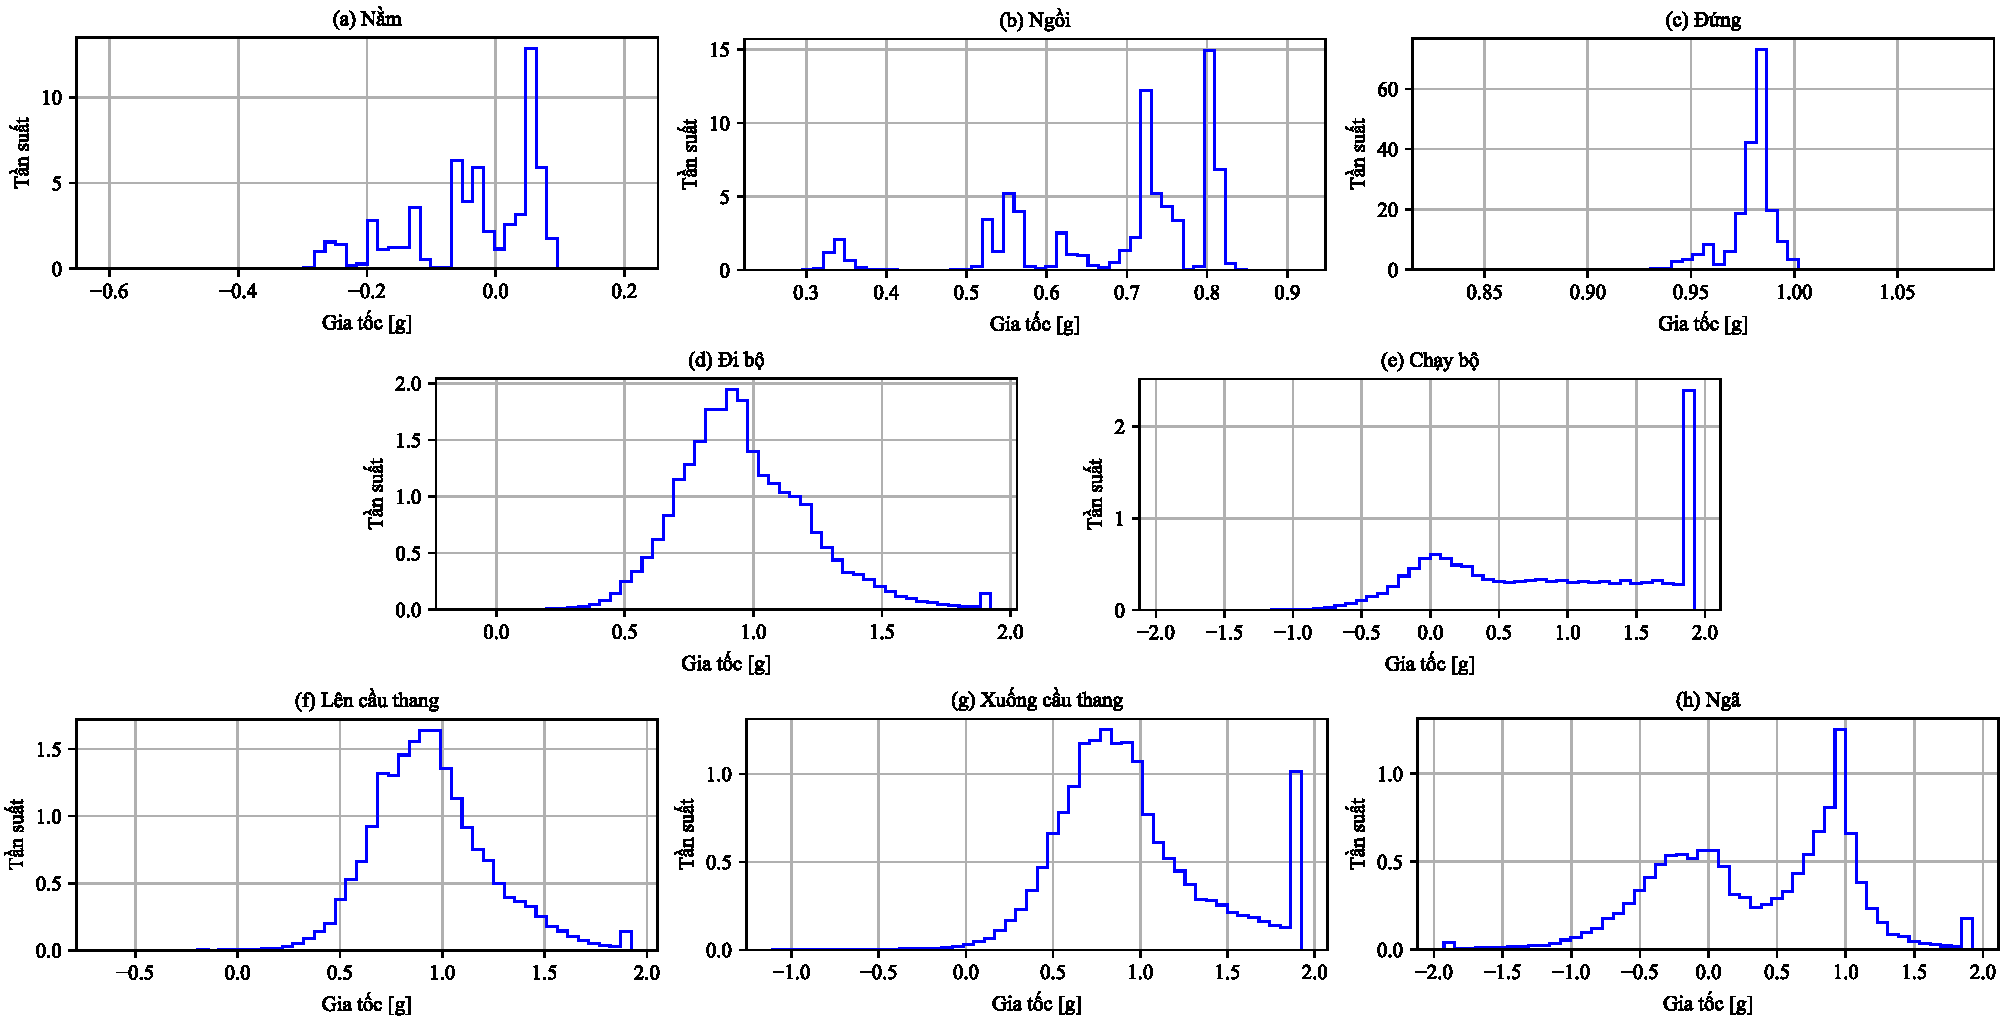
\includegraphics[width=1\linewidth]{Figure/histogram.pdf}
    \caption{Biểu đồ histogram của giá trị gia tốc theo trục $\mathrm{a_x}$ trong tám hành động khác nhau: (a) nằm, (b) ngồi, (c) đứng, (d) đi bộ, (e) chạy bộ, (f) lên cầu thang, (g) xuống cầu thang, và (h) ngã} % Trục hoành biểu diễn giá trị gia tốc (đơn vị: $\text{g}$), trục tung biểu diễn tần suất đã được chuẩn hoá
    \label{histogram}
\end{figure}

\begin{table}[b!]
    \centering
    \caption{Các đặc trưng miền thời gian được trích xuất từ tín hiệu gia tốc và vai trò trong nhận diện hành động}
    \label{feature}
    \begin{tabular}{p{0.126\linewidth}p{0.21\linewidth}p{0.25\linewidth}p{0.31\linewidth}}\hline\hline
        \multicolumn{1}{c}{\textbf{Đặc trưng}} & \multicolumn{1}{c}{\textbf{Công thức}} & \multicolumn{1}{c}{\textbf{Định nghĩa}} & \multicolumn{1}{c}{\textbf{Vai trò}}\\\hline
        
        \multirow{3}{*}{Trung bình} & \multirow{3}{*}{$\mu = \frac{1}{N} \sum_{i=1}^{N} x_i$} & \parbox[t]{\linewidth}{\justifying \noindent Trung bình cộng của tất cả mẫu tín hiệu trong một cửa sổ thời gian.} & Phản ánh xu hướng tổng thể của tín hiệu. Giúp phân biệt giữa các tư thế tĩnh.\\\hline
        
        \multirow{4}{*}{Độ lệch chuẩn} & \multirow{4}{*}{$\sigma = \sqrt{ \frac{1}{N} \sum_{i=1}^{N} (x_i - \mu)^2 }$} & \multirow{4}{*}{\parbox[t]{\linewidth}{\justifying \noindent Mức độ phân tán của tín hiệu quanh giá trị trung bình.}} & Đặc trưng cho mức độ dao động của chuyển động. Cao ở hành động động (chạy, ngã), thấp ở trạng thái tĩnh (đứng, ngồi).\\\hline
        
        \multirow{4}{*}{\parbox[t]{\linewidth}{\justifying \noindent Bình phương trung bình gốc}} & \multirow{4}{*}{$\chi = \sqrt{ \frac{1}{N} \sum_{i=1}^{N} x_i^2 }$} & \multirow{4}{*}{\parbox[t]{\linewidth}{\justifying \noindent RMS đại diện cho năng lượng trung bình của tín hiệu trong một khoảng thời gian.}} & Được sử dụng để đánh giá cường độ chuyển động. RMS cao ở các hành vi có hoạt động mạnh như chạy hoặc ngã.\\\hline
        
        \multirow{4}{*}{Cực đại} & \multirow{4}{*}{$\varkappa = \max(x)$} & \multirow{4}{*}{\parbox[t]{\linewidth}{\justifying \noindent Giá trị lớn nhất của tín hiệu trong một cửa sổ thời gian.}} & Nhạy với biên độ gia tốc lớn, thường xuất hiện trong hành vi có chuyển động mạnh hoặc bất thường.\\\hline
        
        \multirow{4}{*}{Cực tiểu} & \multirow{4}{*}{$\eta = \min(x)$} & \multirow{4}{*}{\parbox[t]{\linewidth}{\justifying \noindent Giá trị nhỏ nhất của tín hiệu trong một cửa sổ thời gian.}} & Kết hợp với cực đại để đánh giá biên độ biến thiên, đặc biệt hữu ích trong các hành vi như ngã hoặc nhảy.\\\hline
        
        \multirow{3}{*}{Phạm vi} & \multirow{3}{*}{$\gamma = \max(x) - \min(x)$} & \multirow{3}{*}{\parbox[t]{\linewidth}{\justifying \noindent Khoảng chênh lệch giữa giá trị lớn nhất và nhỏ nhất.}} & Đặc trưng cho mức độ thay đổi tổng thể; cao trong các hành vi có biên dao động rộng như chạy hoặc ngã.\\\hline
        
        \multirow{3}{*}{Trung vị} & \multirow{3}{*}{$\Psi = \mathrm{median}(x)$} & Giá trị chia phân phối tín hiệu thành hai phần bằng nhau. & Ít bị ảnh hưởng bởi nhiễu; giúp phân biệt hành vi tĩnh với mức dao động nhỏ và ổn định.\\ \hline
        
        \multirow{4}{*}{Tứ phân vị} & \multirow{4}{*}{$\Xi = Q_3 - Q_1$} & \multirow{4}{*}{\parbox[t]{\linewidth}{\justifying \noindent Khoảng giữa của 50~\% giá trị trung tâm, loại bỏ ảnh hưởng của ngoại lai.}} & Phản ánh mức độ phân tán bên trong; hữu ích với hành vi có dao động vừa phải như đi bộ, lên cầu thang.\\
        \hline\hline
    \end{tabular}
\end{table}

Để hiểu rõ hơn cách các đặc trưng này phản ánh bản chất của chuyển động, chúng tôi tiến hành phân tích trực quan phân bố giá trị gia tốc thô qua biểu đồ tần suất (histogram) cho từng hành động. Hình~\ref{histogram} thể hiện biểu đồ histogram của giá trị gia tốc theo trục $\mathrm{a_x}$ trong tám hành động khác nhau: nằm (a), ngồi (b), đứng (c), đi bộ (d), chạy bộ (e), lên cầu thang (f), xuống cầu thang (g), và ngã (h). Các biểu đồ này cung cấp cái nhìn trực quan về phân bố giá trị gia tốc, cho phép phân biệt rõ ràng giữa các hoạt động tĩnh, hoạt động có chu kỳ và hoạt động bất thường.

Các hoạt động tĩnh như nằm, ngồi và đứng (a–c) cho thấy phân bố gia tốc hẹp với giá trị dao động nhỏ quanh một điểm gần cố định. Cụ thể, hành động nằm có giá trị trung bình gần 0~g và phạm vi nhỏ từ khoảng -0,3~g đến 0,2~g, cho thấy ít dao động (độ lệch chuẩn thấp) và đặc trưng bởi các trị trung vị và tứ phân vị gần nhau. Tương tự, ngồi và đứng cho thấy phân bố hẹp hơn, với cực đại gần 1~g cho đứng (c) và khoảng 0,8~g cho ngồi (b). Điều này phản ánh sự ổn định và ít biến thiên, thể hiện rõ qua các đặc trưng như trung bình, độ lệch chuẩn và IQR thấp.

Ngược lại, các hành động động như đi bộ, chạy bộ, lên và xuống cầu thang (d–g) thể hiện phân bố rộng hơn với nhiều dao động, phản ánh bản chất chu kỳ và thay đổi liên tục của chuyển động. Đi bộ (d) và lên cầu thang (f) đều có trung bình khoảng 1~g nhưng có độ lệch chuẩn và khoảng dao động lớn (range rộng từ 0~g đến xấp xỉ 2~g), dẫn đến các đặc trưng như RMS và tứ phân vị cũng tăng cao. Chạy bộ (e) cho thấy phân bố lệch với cực đại rõ rệt tại khoảng 2~g, biểu thị lực va đập mạnh hơn, đồng thời cho thấy sự bất đối xứng trong phân bố—điều này ảnh hưởng đến chênh lệch giữa trung bình và trung vị. Xuống cầu thang (g) cũng có xu hướng dao động mạnh tương tự chạy bộ, nhưng phân bố rộng hơn về phía biên âm (tới -1,2~g), làm tăng giá trị min và range.

Đặc biệt, hành động ngã (h) cho thấy đặc điểm phân bố khác biệt rõ rệt so với các hành vi còn lại. Biểu đồ này thể hiện hai đỉnh rõ rệt, một tại khoảng -1~g và một tại khoảng 1~g, cùng với phạm vi dao động rất rộng từ -2~g đến 2~g. Điều này phản ánh sự biến đổi đột ngột và không chu kỳ trong quá trình ngã—một đặc điểm đặc trưng của gia tốc không kiểm soát. Các đặc trưng thống kê như độ lệch chuẩn, max, min, và range trong trường hợp này đều đạt giá trị cao, trong khi median và IQR có thể dao động mạnh tùy thuộc vào hướng rơi và thời điểm ghi nhận. Những đặc trưng này đóng vai trò then chốt trong việc giúp mô hình học máy phân biệt hành động ngã với các hành động động thông thường.

Tổng thể, sự khác biệt rõ rệt trong phân bố histogram giữa các hành động, khi được mô tả và mã hóa bằng 8 đặc trưng miền thời gian, tạo nên bộ đặc trưng định lượng hiệu quả cho mô hình phân loại hành vi dựa trên cảm biến gia tốc (Bảng~\ref{feature}). Việc phân tích histogram cho phép chúng ta không chỉ hình dung được phân bố của dữ liệu gia tốc cho mỗi hoạt động mà còn cung cấp cơ sở trực quan để hiểu tại sao các đặc trưng thống kê như trung bình, độ lệch chuẩn, RMS, cực đại, cực tiểu, phạm vi, trung vị và IQR lại quan trọng và có khả năng phân biệt cao giữa các lớp hoạt động khác nhau, đặc biệt là trong việc nhận diện sự kiện ngã và các hành vi vận động phức tạp.

\begin{figure}[b!]
    \centering
    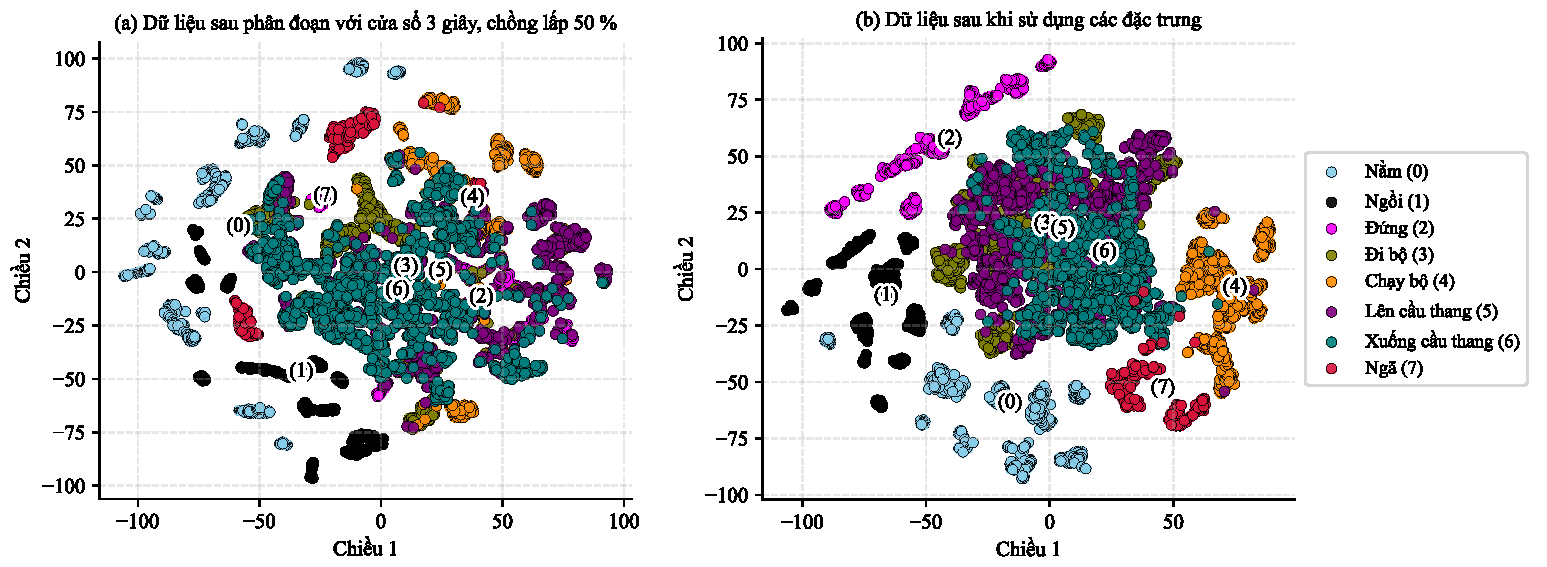
\includegraphics[width=1\linewidth]{Figure/tsne.pdf}
    \caption{Biểu diễn trực quan dữ liệu sử dụng t-SNE: (a) Dữ liệu sau phân đoạn với cửa sổ trượt 3 giây và chồng lấp 50~\%; (b) Dữ liệu sau khi trích xuất đặc trưng thống kê}
    \label{tsne}
\end{figure}

Để đánh giá trực quan khả năng phân tách giữa các hành vi, chúng tôi sử dụng thuật toán t-SNE để biểu diễn dữ liệu trong không gian hai chiều. Hình~\ref{tsne} trình bày kết quả biểu diễn trước và sau khi áp dụng trích xuất đặc trưng. Cụ thể, hình~\ref{tsne}a thể hiện dữ liệu sau phân đoạn nhưng chưa qua trích xuất đặc trưng—cho thấy sự phân bố chồng lấp đáng kể giữa các hành động, gần như không thể phân biệt được. Ngược lại, hình~\ref{tsne}b thể hiện dữ liệu sau khi áp dụng các đặc trưng thống kê, cho thấy sự tách biệt rõ ràng hơn giữa các nhóm hành vi.

Tuy nhiên, có thể quan sát thấy vẫn còn một số mức độ chồng lấp giữa các hành vi vận động như đi bộ, chạy bộ, và lên/xuống cầu thang. Kết quả này phù hợp với quan sát từ histogram, nơi mà các hành động kể trên có đặc trưng phân bố tương tự nhau: đều có biên độ dao động cao, mang tính chu kỳ, và phạm vi dao động gần nhau trên trục gia tốc. Do đó, việc nhầm lẫn giữa các hành vi này là điều dễ hiểu và được phản ánh trong không gian đặc trưng.

\subsubsection{Chiến lược lựa chọn và đánh giá mô hình}

Việc lựa chọn mô hình học máy phù hợp luôn là một trong những bước then chốt và khó khăn nhất trong quá trình phát triển hệ thống phân loại, đặc biệt là trong các bài toán phân lớp nhiều nhãn như nhận dạng hành động và phát hiện ngã. Khác với các mô hình học sâu, vốn tập trung vào việc tinh chỉnh kiến trúc mạng (như số tầng, loại tầng), học máy truyền thống đòi hỏi sự phân tích kỹ lưỡng về không gian đặc trưng, số chiều dữ liệu, giả định phân phối, cũng như hành vi của mô hình dưới các tổ hợp siêu tham số khác nhau. Điều này càng trở nên quan trọng hơn khi mô hình cần triển khai trên các thiết bị nhúng hiệu năng thấp, vốn bị giới hạn nghiêm ngặt về bộ nhớ và tài nguyên tính toán.

Trong khi nhiều nghiên cứu trước đây so sánh các bộ phân loại học máy nhằm làm nổi bật hiệu suất của mô hình chính mà họ lựa chọn—nhưng lại không cung cấp thông tin cụ thể về quá trình lựa chọn siêu tham số, hoặc thậm chí hoàn toàn bỏ qua bước này~\cite{vi2024efficient}, \cite{chen2019detection}—thì nghiên cứu này đề xuất một quy trình đánh giá có kiểm soát chặt chẽ nhằm đảm bảo tính khách quan và khả năng tái lập kết quả. Thực tế, không ít nghiên cứu lựa chọn một mô hình chính (ví dụ như RF), sau đó so sánh với các mô hình khác như GBDT, SVM, hoặc KNN mà không làm rõ cách thiết lập hoặc lựa chọn siêu tham số tương ứng cho các mô hình được đem ra so sánh~\cite{bui2024smart}, \cite{hong2023low}, \cite{dao2022human}, \cite{thu2022real}. Cách tiếp cận này tiềm ẩn nguy cơ đánh giá thiên lệch hiệu suất, đặc biệt khi các mô hình được đặt cạnh nhau mà không tuân theo một tiêu chí thống nhất trong thiết lập và đánh giá—từ đó ảnh hưởng đến độ tin cậy và khả năng tái lập của kết quả nghiên cứu.

Trong nghiên cứu này, chúng tôi áp dụng quy trình xác thực chéo lồng nhau (Nested Cross-Validation - NCV), kết hợp với xác thực chéo tiêu chuẩn (Vanilla Cross-Validation - VCV), nhằm đạt được cả hai mục tiêu: (i) đánh giá công bằng ước tính hiệu suất không thiên vị của các mô hình dưới điều kiện giống nhau; và (ii) lựa chọn chính xác siêu tham số cuối cùng cho mô hình triển khai. Ở bước đầu tiên, NCV được sử dụng để đánh giá hiệu suất tổng thể của năm bộ phân loại: Extra Trees (ET), Gradient Boosting Decision Trees (GBDT), Light Gradient Boosting Machine (LightGBM), Random Forest (RF) và Extreme Gradient Boosting (XGBoost). Tất cả các bộ phân loại đều chia sẻ cùng một không gian siêu tham số nhằm đảm bảo công bằng trong quá trình so sánh: \texttt{n\_estimators} được quét từ 1 đến 30, \texttt{max\_depth} từ 1 đến 20, và toàn bộ quy trình đặt \texttt{random\_state} $=$ 42 để đảm bảo tái lập.

\begin{table}[b!]
    \centering
    \caption{Số lượng cửa sổ dữ liệu hành động trong NCV trên tập riêng tư}
    \label{nested_cv_har}
    \begin{tabular}{llrr}\hline\hline
        \textbf{Vòng lặp ngoài (10 fold)} & \textbf{Vòng lặp trong (10 fold)} &  & \textbf{Tổng}\\\hline
        \multirow{2}{*}{Huấn luyện} & Huấn luyện & 7.929 & \multirow{2}{*}{8.811}\\\cline{2-3}
         & Xác thực & 882 & \\\hline
        Kiểm tra &  &  & 979\\\hline
        Tổng &  &  & 9.790\\\hline\hline
    \end{tabular}
\end{table}

\begin{table}[b!]
    \centering
    \caption{So sánh hiệu suất và kích thước mô hình của các bộ phân loại theo quy trình NCV và VCV}
    \label{hyperparameter}
    \begin{tabular}{>{\raggedright\arraybackslash}p{0.09\linewidth}>{\centering\arraybackslash}p{0.195\linewidth}>{\centering\arraybackslash}p{0.126\linewidth}||>{\centering\arraybackslash}p{0.18\linewidth}>{\centering\arraybackslash}p{0.124\linewidth}>{\centering\arraybackslash}p{0.125\linewidth}}\hline\hline
        \multirow{3}{*}{\textbf{Bộ phân loại}} & \multirow{3}{*}{\textbf{Cấu hình}} & \textbf{Nested CV} & \multicolumn{3}{c}{\textbf{Vanilla CV}}\\\cline{3-6}
         &  & \makecell[t]{\textbf{F1\textsubscript{macro}} \\ \textbf{(\%)}} & \multirow{2}{*}{\textbf{Siêu tham số}} & \makecell[t]{\textbf{F1\textsubscript{macro}} \\ \textbf{(\%)}} & \makecell[t]{\textbf{Dung lượng} \\ \textbf{(kB)}}\textsuperscript{$\vee$}\\\hline
        
        \multirow{2}{*}{ET} & \multirow{10}{*}{\makecell{$\mathrm{n\_estimators} \in$ [1, 30], \\ \hspace{0.45em} $\mathrm{max\_depth} \in$ [1, 20], \\ \hspace{-0.15em} $\mathrm{random\_state}=$ 42}} & \multirow{2}{*}{98,18 $\pm$ 0,38} & \cellcolor{green!50} \makecell[t]{$\mathrm{n\_estimators}=$ 11,\\ \hspace{0.20em} $\mathrm{max\_depth}=$ 12} & \cellcolor{green!50} \multirow{2}{*}{96,57 $\pm$ 0,44} & \cellcolor{green!50} \multirow{2}{*}{987}\\\cline{1-1} \cline{3-6}
        
        \multirow{2}{*}{GBDT} &  & \multirow{2}{*}{98,00 $\pm$ 0,36} & \cellcolor{orange!50} \makecell[t]{$\mathrm{n\_estimators}=$ 30,\\ \hspace{0.20em} $\mathrm{max\_depth}=$ 05} & \cellcolor{orange!50} \multirow{2}{*}{97,82 $\pm$ 0,34} & \cellcolor{orange!50} \multirow{2}{*}{1.020}\\\cline{1-1} \cline{3-6}
        
        \multirow{2}{*}{LightGBM} &  & \multirow{2}{*}{98,22 $\pm$ 0,56} & \cellcolor{green!50} \makecell[t]{$\mathrm{n\_estimators}=$ 24,\\ \hspace{0.20em} $\mathrm{max\_depth}=$ 08} & \cellcolor{green!50} \multirow{2}{*}{98,02 $\pm$ 0,49} & \cellcolor{green!50} \multirow{2}{*}{993}\\\cline{1-1} \cline{3-6}
        
        \multirow{2}{*}{RF} &  & \multirow{2}{*}{98,10 $\pm$ 0,27} & \cellcolor{cyan!50} \makecell[t]{$\mathrm{n\_estimators}=$ 13,\\ \hspace{0.20em} $\mathrm{max\_depth}=$ 12} & \cellcolor{cyan!50} \multirow{2}{*}{97,55 $\pm$ 0,34} & \cellcolor{cyan!50} \multirow{2}{*}{1.001}\\\cline{1-1} \cline{3-6}
        
        \multirow{2}{*}{XGBoost} &  & \multirow{2}{*}{98,38 $\pm$ 0,40} & \cellcolor{cyan!50} \makecell[t]{$\mathrm{n\_estimators}=$ 30,\\ \hspace{0.20em} $\mathrm{max\_depth}=$ 06} & \cellcolor{cyan!50} \multirow{2}{*}{98,38 $\pm$ 0,35} & \cellcolor{cyan!50} \multirow{2}{*}{\textbf{866}}\\\hline\hline
    \end{tabular}
\vspace{0.2em}\\
\justifying\noindent \textsuperscript{$\vee$}Chuyển đổi mô hình sang mã C/C++: \! \colorbox{green!50}{\tiny\phantom{X}} m2cgen, \colorbox{orange!50}{\tiny\phantom{X}} Phân rã cây + m2cgen, \colorbox{cyan!50}{\tiny\phantom{X}} micromlgen
\end{table}

Trong cấu trúc NCV, vòng lặp trong (inner loop) thực hiện tìm kiếm tổ hợp siêu tham số tối ưu bằng phương pháp GridSearch, trong khi vòng lặp ngoài (outer loop) dùng để đánh giá hiệu suất của mô hình ứng với các siêu tham số đã được chọn. Cách tiếp cận này giúp giảm thiểu nguy cơ overfitting, đảm bảo mô hình được đánh giá trên các tập dữ liệu chưa từng được sử dụng trong quá trình tối ưu và mang lại đánh giá khách quan hơn về hiệu suất tổng quát hóa của mô hình. Cấu trúc NCV được thực hiện theo 10-fold cho cả inner và outer loop, với tổng cộng 9.790 cửa sổ dữ liệu đầu vào, bao gồm 7.929 cửa sổ huấn luyện, 882 cửa sổ xác thực và 979 cửa sổ kiểm thử (Bảng~\ref{nested_cv_har}). Với không gian siêu tham số như trên, NCV đã thực hiện tổng cộng 30 $\times$ 20 $\times$ 10 $\times$ 10 $=$ 60.000 lượt huấn luyện mô hình. Để đáp ứng yêu cầu tính toán này, chúng tôi sử dụng máy chủ Dell PowerEdge T550 với bộ vi xử lý Intel Xeon Silver 4310.

Kết quả đánh giá hiệu suất của năm bộ phân loại trên tập dữ liệu riêng tư thông qua NCV được trình bày trong bảng~\ref{hyperparameter}. Trong đó, XGBoost đạt F1\textsubscript{macro} trung bình cao nhất (98,38~\%), tiếp theo là LightGBM (98,22~\%), ET (98,18~\%), RF (98,10~\%) và cuối cùng là GBDT (98,00~\%). Các mô hình đều được đánh giá dưới cùng một không gian siêu tham số và tiêu chí lặp lại để đảm bảo công bằng trong quá trình so sánh.

\begin{figure}[b!]
    \centering
    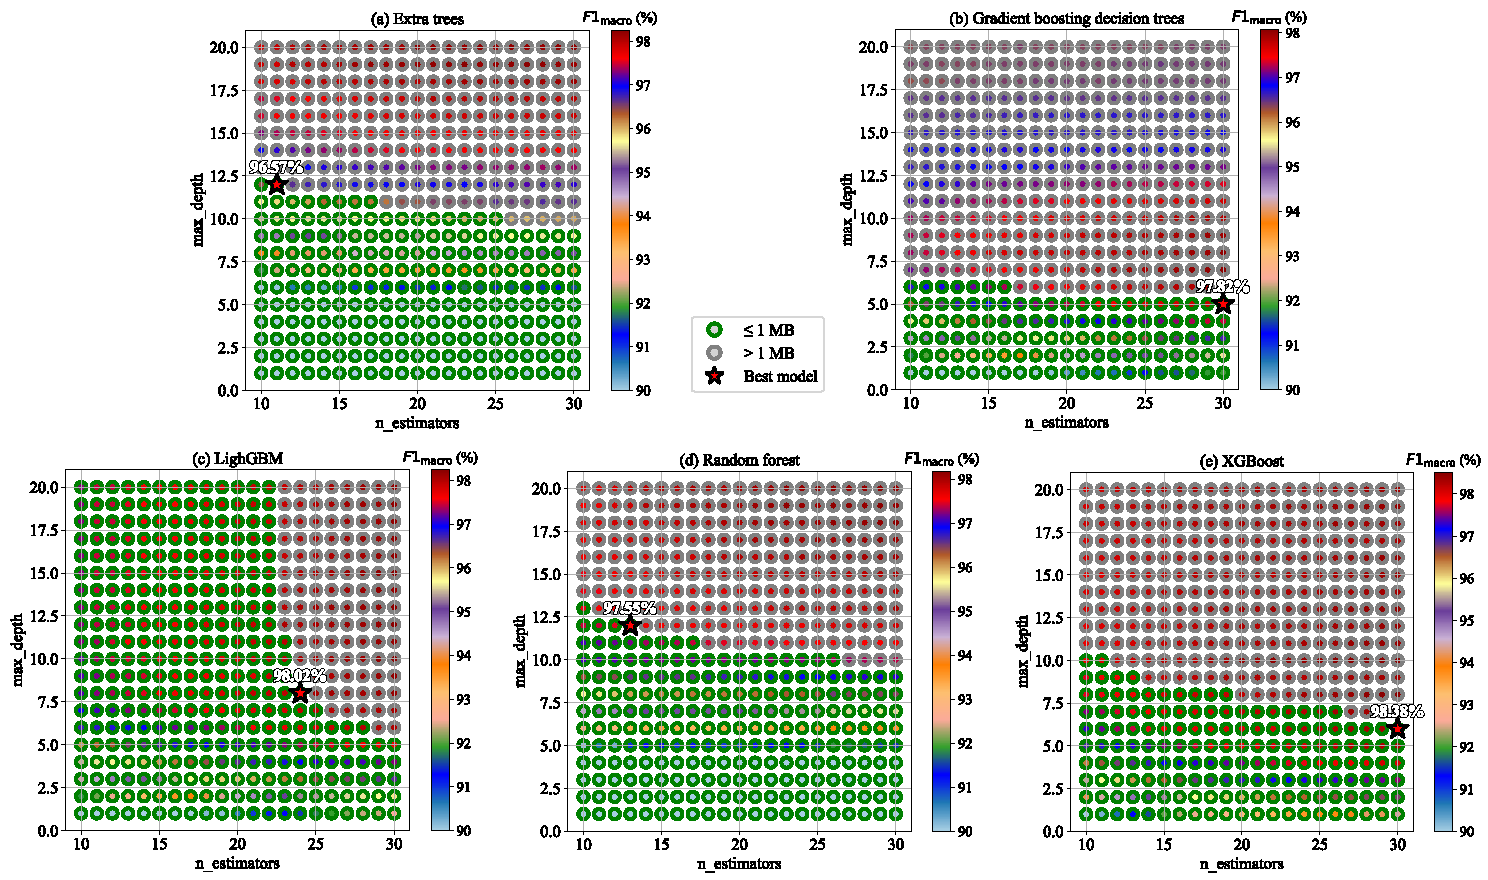
\includegraphics[width=1\linewidth]{Figure/heatmap.pdf}
    \caption{Bản đồ nhiệt về hiệu suất phân loại và kích thước mô hình trong quá trình xác thực chéo}
    \label{heatmap}
\end{figure}

Ở bước thứ hai, chúng tôi sử dụng VCV để xác định tổ hợp siêu tham số tối ưu cuối cùng cho từng mô hình. Với mỗi tổ hợp được chọn, mô hình được huấn luyện trên toàn bộ dữ liệu huấn luyện và được chuyển đổi sang mã C/C++ bằng thư viện \texttt{m2cgen} hoặc \texttt{micromlgen} để đo lường kích thước thực tế.

Kết quả cho thấy trong số nhiều mô hình ứng viên, XGBoost đạt điểm F1\textsubscript{macro} cao nhất là 98,38~\%, vượt trội so với các đối thủ. Quan trọng hơn, bản đồ nhiệt tối ưu hóa tham số (Hình~\ref{heatmap}) minh họa cách cấu hình được chọn với \texttt{n\_estimators} $=$ 30 và \texttt{max\_depth} $=$ 6 không chỉ cung cấp độ chính xác phân loại hàng đầu mà còn tạo ra kích thước mô hình nhỏ gọn là 866~kB, thấp hơn so với bốn bộ phân loại khác và so với giới hạn bộ nhớ Flash 1~MB thông thường của các MCU mục tiêu. Điều này cho phép hệ thống thực hiện suy luận thời gian thực đáng tin cậy trong phạm vi tài nguyên tính toán và bộ nhớ hạn chế hiện có. Đây là một yếu tố then chốt trong bối cảnh tài nguyên hệ thống bị giới hạn nghiêm ngặt: một vi điều khiển điển hình chỉ có khoảng 128 đến 256~kB RAM và 1~MB bộ nhớ Flash, trong khi một điện thoại di động có thể có 4~GB RAM và 64~GB bộ nhớ lưu trữ. Do đó, việc cân bằng giữa độ chính xác, độ phức tạp mô hình và giới hạn tài nguyên là một yếu tố sống còn khi triển khai hệ thống HAR trên LPMC.

Từ các phân tích trên, chúng tôi lựa chọn XGBoost là mô hình triển khai cuối cùng trong hệ thống, với số lượng cây tăng cường là 30 và độ sâu tối đa của mỗi cây là 6, vì đây là phương án cân bằng tối ưu giữa độ chính xác cao, độ phức tạp mô hình hợp lý và khả năng triển khai thực tế trên nền tảng vi điều khiển hiệu suất thấp. Mô hình đã được huấn luyện được biên dịch thành thư viện C/C++ nhúng, với tất cả các tham số được lưu trữ trong bộ nhớ Flash để thực thi trên thiết bị.

\subsubsection{Triển khai nhúng trên vi điều khiển}

ESP32-WROOM-32U, theo thông số của nhà sản xuất, sở hữu 520~kB RAM, 448~kB ROM và 4~MB Flash. Tuy nhiên, ROM phần lớn dành cho mã hệ thống, bao gồm bộ nạp khởi động và các giao thức mạng, trong khi Flash phải chia sẻ dung lượng cho firmware, phân vùng cập nhật OTA và hệ thống tệp, dẫn đến dung lượng khả dụng cho mã chương trình và mô hình chỉ vào khoảng 2–2.5~MB. Bên cạnh đó, sau khi cấp phát bộ nhớ cho ngăn xếp Wi-Fi, hệ điều hành và các tiến trình nền, dung lượng RAM còn lại cho nhiệm vụ ứng dụng vào khoảng 320–400~kB. Do đó, việc nhúng mô hình học máy vào ESP32 phải cân nhắc kỹ về chiến lược lưu trữ trọng số, ưu tiên đặt chúng trong bộ nhớ Flash và hạn chế sử dụng RAM để dành cho các tác vụ xử lý dữ liệu thời gian thực.

Quy trình triển khai mô hình XGBoost bao gồm các bước huấn luyện, chuyển đổi và tích hợp. Sau khi huấn luyện và tinh chỉnh trên môi trường máy tính, mô hình được xuất sang mã C/C++ thông qua thư viện \texttt{micromlgen}, cho phép chuyển đổi toàn bộ cấu trúc cây và trọng số thành các hằng số có thể nạp trực tiếp vào bộ nhớ Flash của vi điều khiển. Mô hình được tích hợp vào firmware thông qua tệp tiêu đề (\texttt{model\_XGB.h}) và gọi bằng lớp \texttt{Eloquent::ML::Port::XGBClassifier model\_XGB}. Trong quá trình suy luận trên vi điều khiển, dữ liệu cảm biến từ GY-85 được xử lý theo cửa sổ trượt 3 giây với độ chồng lấp 50~\%, tức sau mỗi 1,5 giây hệ thống cập nhật trạng thái dựa trên 150 mẫu dữ liệu mới kết hợp với 150 mẫu dữ liệu từ cửa sổ trước. Tập đặc trưng thu được từ cửa sổ này được chuẩn hóa và đưa vào mô hình XGBoost để dự đoán nhãn hành động. Kết quả dự đoán sau đó được sử dụng để kích hoạt các chức năng phản hồi, bao gồm gửi cảnh báo đến trung tâm chỉ huy.

\begin{figure}[b!]
    \centering
    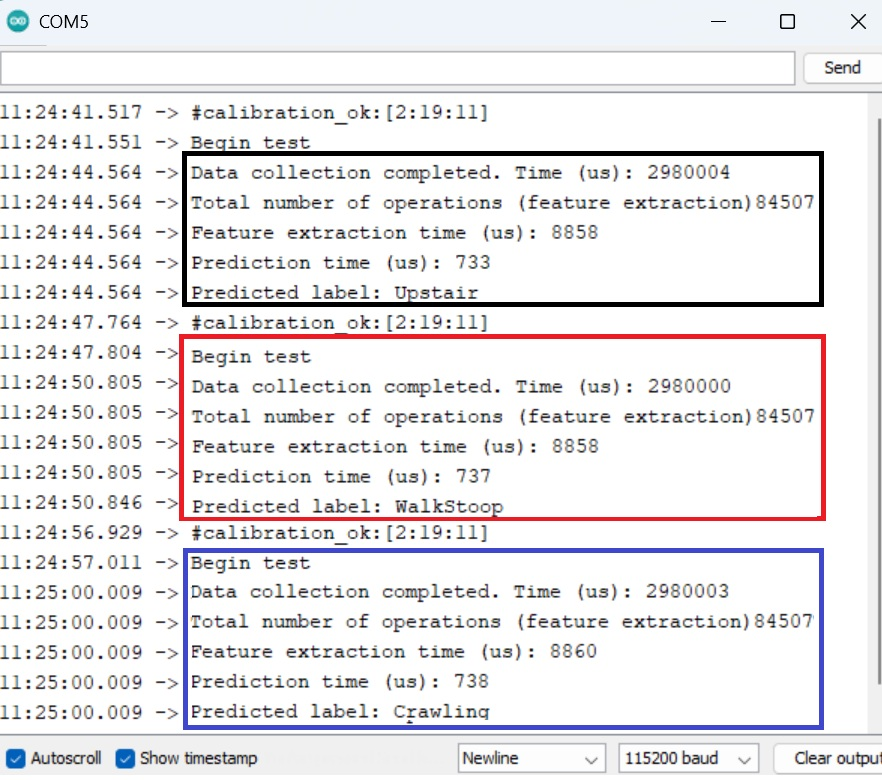
\includegraphics[width=0.77\linewidth]{Figure/Suyluan.png}
    \caption{Kết quả triển khai nhận dạng trên vi điều khiển}
    \label{Suyluan}
\end{figure}

Hình~\ref{Suyluan} cho thấy thời gian thực tế và thời gian tính toán trên vi điều khiển cho từng giai đoạn xử lý, bao gồm thu thập dữ liệu, trích xuất đặc trưng và nhận dạng. Với thiết bị đeo tích hợp vi điều khiển ESP32 và cảm biến gia tốc ADXL345, quy trình xử lý từ đầu đến cuối đã được đánh giá để đảm bảo khả năng hoạt động thời gian thực. Trong quá trình hoạt động, cảm biến gia tốc lấy mẫu dữ liệu ba trục ở tần số 100~Hz, và hệ thống thu thập 900 mẫu trong khoảng thời gian 3 giây. Sau khi hoàn tất thu thập dữ liệu, quá trình trích xuất đặc trưng được thực hiện với khoảng 84.507 dòng lệnh, mất khoảng 8,858~µs. Mô hình được đề xuất, với 140.838 dòng lệnh, thực hiện suy luận trong khoảng 733–738~µs. Sau khi nhận dạng, kết quả nhận dạng được truyền qua SPI ở tốc độ 10 MHz, mất chỉ khoảng 1,6~µs và có thể xem là không đáng kể.